\documentclass[12pt, a4paper]{article}

\usepackage{graphicx}
\usepackage{gensymb}
\usepackage[margin=1in]{geometry}
\usepackage{underscore}
\usepackage{amsmath}
\usepackage{subcaption}

\usepackage{hyperref}

\begin{document}

\title{Reconstructing an RGB image from a Sinogram}
\author{Darragh Glavin, Lorcan Williamson, Yilin Mou}
\maketitle


\section*{Introduction}
	A sinogram is a visual representation of the radon transform. It is made up of 1D projections of a 2D image taken at various angles $\theta \in \{0\degree, ..., 180\degree\}$. By stacking the scans taken of an object over a range of angles, a sinogram can be built up (Fig. \ref{fig:sinogram}). As they are mainly used in medical imaging they are normally single-channel images (grayscale). However multi-channel, RGB, sinograms can still be constructed by applying the radon transform to each channel separately.
	
	\begin{figure}[h]
		\centering
		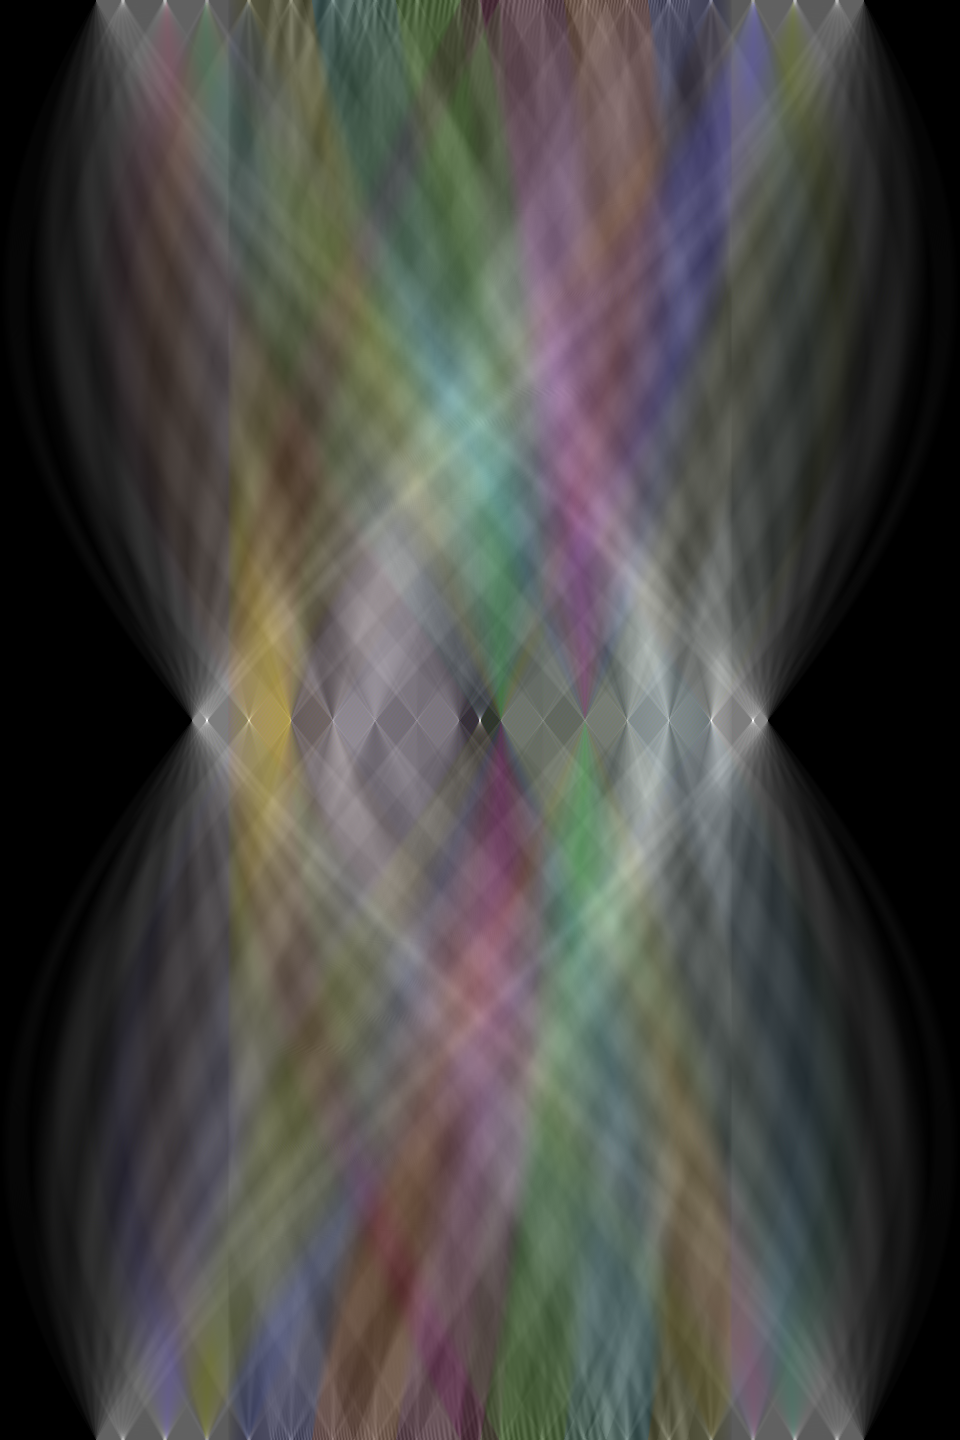
\includegraphics[height=0.4\textheight]{../sinogram.png}
		\caption{RGB Sinogram used for this project}
		\label{fig:sinogram}
	\end{figure}
	
\section*{Methodology}
	As a sinogram is just a visual representation of the radon transform, the original image should be recoverable by using an inverse radon transform. However due to practical limitations a sinogram is constructed using a discrete radon transform, and some information is lost. This means simply applying an inverse radon transform will recover a very noisy image. There are ways however to reduce this noise, namely through the use of the Fourier transform and filtering. For this project therefore, 3 different image recovery methods were looked at;
	\begin{itemize}
		\item \textbf{Inverse Radon Transform:} Just applying the inverse radon transform, i.e. a sum of rotated back-projections.
		\item \textbf{Ramp-filtering:} By applying a ramp filter some of the noise introduced by the radon transform can be removed. This filter was applied by first moving the image to the frequency domain through the use of the Fourier transform, before multiplying by a ramp function. This removed the need for convolution, a relatively computationally expensive function.
		\item \textbf{Windowing:} By applying a windowing function, such as the Hamming or Hann window function, before processing the final image should be 'smoother', as more of the dominant frequencies will be retained after converting the image to the frequency domain, and the noise suppressed.
	\end{itemize}
	After the image was recovered it then needed to be cropped and the pixel values rescaled to make $I[r, c] \in \{0,...,255\}\ \forall\ [r, c]$. It was decided to make each of these steps a distinct function take takes the image as its only input, and return some transformation on the image. This allowed for a simple pipeline of steps to be made, through which each channel could be passed. Functionality was also added to this pipe-lining to allow for the intermediate results to be recorded for debugging and report writing. Using a pipeline also allowed for multi-threading to be used to process the 3 channels simultaneously.
	
\section*{Reconstruction Without Filtering}
	The first method looked at was reconstructing the image simply by summing together the rotated back-projections. This required 3 steps;
	\begin{enumerate}
		\item Summing together of the back-projections after rotating each to its corresponding angle.
		\item Cropping of the image.
		\item Rescaling of the pixel values.
	\end{enumerate}
	Each of these was made into its own function, and will be talked through here.
	\subsubsection*{Reconstruction of Original Image}
	As mentioned a sinogram consists of a number of 1-d scans taken of an object over a range of angles. By extruding these 1-d projections into 2-d back-projections, and rotating them back to their original angle, the view of the sensor at that angle can be recovered. Doing this for all angles and summing them together will result in a reconstruction of the original image. This also means some information about the original object can be easily read from the sinogram, namely the number of angles scans were taken at, and the maximum cross-sectional width of the object, which correspond to the number of rows and number of columns in the sinogram respectively. \\
	To form these back-projections NumPy's \texttt{tile} function was used. This function takes a NumPy array and projects it to a new shape. As we know that all the back-projections must be square, we can simply project each row $r$ of the sinogram from shape $1 \times c$ to $c \times c$. Then each back-projection is then rotated by $\Delta\theta \times r$, where $\Delta\theta$ is equal to $180^\circ$ divided by the number of rows in the sinogram, to the blank image. The rotations where done using skimage's $rotate$ function. These are then added together to form a laminogram. The result of this can be seen in Figure \ref{fig:no-filter-un-cropped}. \\
	
	\begin{figure}
		\centering
		\includegraphics[width=0.7\textwidth]{./images/no-filter-un-cropped.png}
		\caption{Un-cropped laminogram (Pixel values rescaled)}
		\label{fig:no-filter-un-cropped}
	\end{figure}
	
	\subsubsection*{Cropping}
	This laminogram must then be cropped to recover the original image. Using the fact that original image is rectangular and the aspect ratio of it is known to be $4:3$ this can be done relatively simply. The nature of how sinograms are formed means that the original image's widest point, i.e. the diagonal, must correspond to width of the sinogram. This leaves a circle in the center of the recovered image of radius $d$ that the original image resides within, as can be seen in Figure \ref{fig:no-filter-un-cropped}. Using some simple geometry (Eqn. \ref{eqn:cropping}) the dimensions $r \times c$ of the original image can be found. The original image can then be retrieved by taking a slice of this size around the centre of the recovered image, as seen in Figure \ref{fig:no-filter-cropped}.
	
	\begin{align}
		d^2 &= r^2 + c^2, \quad c = \frac{4}{3}r \\
		d^2 &= r^2(1 + (\frac{4}{3})^2) \\
		r &= \frac{d}{\sqrt{(1 + (\frac{4}{3}))^2}} 
		\label{eqn:cropping}
	\end{align}
	
	\begin{figure}
		\centering
		\includegraphics[width=0.7\textwidth]{./images/no-filter-cropped.png}
		\caption{Cropped recovered image (Pixel values rescaled)}
		\label{fig:no-filter-cropped}
	\end{figure}
	
	\subsubsection*{Rescaling}
	The last thing that must be done to fully recover the image to a viewable state is to rescale the pixel values. After summing the back-projections the pixel values can be quite large. For these to be properly viewable they must therefore be converted to an integer value in the range $\{0, ..., 255\}$ \footnote{Other pixel value standards do exist but 8-bit values were used for this project}. This is done according to Equation \ref{eqn:rescale}.

	\begin{equation}
		I[r, c]^\prime = \frac{I[r, c] - I_{min}}{I_{max} - I_{min}} \quad \forall \ [r, c] \in I
		\label{eqn:rescale}
	\end{equation}		
	
\section*{Reconstruction using Ramp Filter}
	As you can see simply using the inverse radon transform to recover the image results in the recovered image being quite blurry. To try and resolve this reconstruction in the frequency domain was looked at. Looking at the 2-D Fourier transform it can be shown that the original image is the sum of the back-projections convolved with a filter, that has a ramp representation in the frequency domain\footnote{For brevity this derivation is not included}(Eqn. \ref{eqn:ramp-filter}). The properties of the Fourier transform mean convolution in the time is equivalent to multiplication in the frequency domain. This property is good for two reasons: multiplication is computationally far cheaper than convolution; and there is no finite spatial-domain representation of a frequency domain ramp.
	
	\begin{equation}
		f(x, y) = \int_{0}^{\pi}\left[ \int_{-\infty}^{\infty} |\omega|G(\omega, \theta) e^{j2\pi\omega\rho} d\omega \right]_{\rho=x\cos\theta + y\sin\theta} d\theta
	\label{eqn:ramp-filter}
	\end{equation}
	
	\newpage
	\noindent
	This led to three new functions being made to carry this out:
	\begin{itemize}
		\item \textbf{\texttt{apply_fft(sinogram)}}: Applies the fast Fourier transform to each row in the sinogram using SciPy's \texttt{rfft} function.
		\item \textbf{\texttt{apply_ramp_filter(sinogram_fft)}}: Multiplies the frequency domain projections (sinogram) by a ramp filter, $|\omega|$.
		\item \textbf{\texttt{apply_inverse_fft(sinogram_fft)}}: Applies the inverse fast Fourier transform to the frequency domain sinogram to transform it back to the spatial domain.
	\end{itemize}
	After applying these three steps the laminogram can be formed as before, and the original image recovered from it by cropping and then rescaling it. Figure \ref{fig:ramp-filtered-cropped} shows the result of this. Of note is that the image is now much clearer. However some reconstruction artefacts are still present.
	
	\begin{figure}[h]
		\centering
		\includegraphics[width=0.7\textwidth]{./images/ramp-filter-cropped.png}
		\caption{Recovered image using ramp filtered}
		\label{fig:ramp-filtered-cropped}
	\end{figure}
	
	\section*{Windowed Ramp Filter}
	These reconstruction artefacts are a common problem when using the FFT, and windowing is used to address this. The standard window function function for this is a raised cosine (Eqn. \ref{eqn:raised-cosine}), for which two values of $\alpha$ are significant; $\alpha=0.54$, and $\alpha=0.5$. These values correspond to the Hamming and Hann window functions, which are the two whose use will be looked at in this section. 
	
	\begin{equation}
		H(\omega) = \alpha + (1 - \alpha)\cos\left(\frac{\omega\pi}{\omega_n}\right)
		\label{eqn:raised-cosine}
	\end{equation}
	
	\noindent
	By multiplying the frequency domain ramp filter by one of these windows functions, the reconstruction artefacts can be significantly reduced, as seen in Figure \ref{fig:ramp-hamming}). 
	
	\begin{figure}[t]
		\centering
		\begin{subfigure}[t]{0.5\textwidth}
			\centering
			\includegraphics[width=\textwidth]{./images/ramp-filter-cropped.png}
			\caption{Ramp filter}
		\end{subfigure}%
		\begin{subfigure}[t]{0.5\textwidth}
			\centering
			\includegraphics[width=\textwidth]{./images/hamming-window-cropped.png}
			\caption{Hamming windowed ramp filter}
		\end{subfigure}
		\caption{Reconstruction using Hamming and Hann windowing}
		\label{fig:ramp-hamming}
	\end{figure}
	Due to the similarity between the Hamming and Hann window functions, the reconstructed images are nearly identical (Figure \ref{fig:hamm-hann}). The only difference being the Hann window function being marginally darker, as it has a slightly smaller $\alpha$ (0.5 vs. 0.54).
	
	\begin{figure}[h]
		\centering
		\begin{subfigure}[t]{0.5\textwidth}
			\centering
			\includegraphics[width=\textwidth]{./images/hamming-window-cropped.png}
			\caption{Hamming window}
		\end{subfigure}%
		\begin{subfigure}[t]{0.5\textwidth}
			\centering
			\includegraphics[width=\textwidth]{./images/hann-window-cropped.png}
			\caption{Hann window}
		\end{subfigure}
		\caption{Reconstruction using Hamming and Hann windowing}
		\label{fig:hamm-hann}
	\end{figure}
	
	\section*{Conclusions}
	This report shows how by using the reverse radon transform, an image can be reconstructed from its sinogram. It shows how a laminogram is formed through the summation of rotated back-projections. The use of frequency domain reconstruction was also looked at as a way to reduce the blurriness seen from simply summing the back-projections. By multiplying the sinogram with a ramp filter in the frequency domain, this blurriness was almost completely removed. However other artefacts still remained due to the reconstruction. To remove these, a raised cosine window function was used. This removed most of the artefacts, and some more of the blurriness. Figure \ref{fig:hamming-original} shows the image reconstructed using the Hamaming windowed ramp filter compared to a copy of the image taken from the web. Comparing them it can be seen that some blurriness is still present, however it is a very close reconstruction of the original.
	
	\begin{figure}[h]
		\centering
		\begin{subfigure}[t]{0.5\textwidth}
			\centering
			\includegraphics[width=\textwidth]{./images/hamming-window-cropped.png}
			\caption{Hamming windowed ramp filter reconstruction}
		\end{subfigure}%
		\begin{subfigure}[t]{0.5\textwidth}
			\centering
			\includegraphics[width=\textwidth]{./images/original-padded.png}
			\caption{Copy of the original image}
		\end{subfigure}
		\caption{Comparison between reconstructed image (a) and a copy of the original (b)}
		\label{fig:hamming-original}
	\end{figure}
	
\end{document}